\documentclass[letterpaper, titlepage, 11pt]{article}
\usepackage{fullpage}
\usepackage{graphicx}
\usepackage{hyperref}
\usepackage{url}
\usepackage{titling}

% This is here so we can have a fancier title page than LaTeX gives us by default
\newcommand{\department}[1]{%
  \gdef\dept{#1}}
\newcommand{\dept}{}
\renewcommand{\maketitlehookd}{%
\par\noindent \dept }

\title{
	smrt: A 3D Media Center User Interface
	\\
	Design
}
\author{
	Cory Maccarrone  \\ {\small \href{mailto:Cory.Maccarrone@colorado.edu}{Cory.Maccarrone@colorado.edu}}
	\and
	Daniel Seikaly   \\ {\small \href{mailto:Daniel.Seikaly@colorado.edu}{Daniel.Seikaly@colorado.edu}}
	\and
	Evan Sheehan     \\ {\small \href{mailto:Wallace.Sheehan@gmail.com}{Wallace.Sheehan@gmail.com}}
	\and
	David Trowbridge \\ {\small \href{mailto:trowbrds@gmail.com}{trowbrds@gmail.com}}
}
\date{December 2, 2005}
\department{
\begin{center}
	CSCI 4308-4318. Software Engineering Project 1 \& 2 \\
	Department of Computer Science \\
	University of Colorado at Boulder \\
	2005-2006 \\
	\vspace{1.5em}
	Sun Microsystems \\
	Santa Clara, CA \\
	\vspace{1em}
	Paul Byrne \\
	{\small \href{mailto:Paul.Byrne@Sun.COM}{Paul.Byrne@Sun.COM}} \\
	\vspace{1em}
	Hideya Kawahara \\
	{\small \href{mailto:Hideya.Kawahara@Sun.COM}{Hideya.Kawahara@Sun.COM}}
\end{center}
}

\begin{document}
\maketitle

\raggedbottom

\pagenumbering{roman}

\hspace{1em}
\pagebreak

\tableofcontents

\pagebreak
\hspace{1em}
\pagebreak

\listoffigures
\pagebreak

\hspace{1em}
\pagebreak

\pagenumbering{arabic}

\section{Project Proposal}
Project Looking Glass is an open source development project based on and evolved
from Sun Microsystems' advanced technology project. It supports running unmodified
existing applications in a 3D space, as well as APIs for 3D window manager and
application development. Project Looking Glass has great potential for allowing
users to look at data in new ways from which they will be able to extract more
information.

The goal of this project is to explore the use of a 3D user interface for home media
centers for use with a TV (and possibly HDTV) display -- think 3D user interface for
TiVo. The main objective is to explore the UI possibilities, so this could be a
mockup or the team may want to integrate with an existing system such as MythTV.

\begin{flushleft}
Interesting areas to explore would be:
\begin{itemize}
\item the selection of programs to record
\item managing conflict of scheduled recordings
\item selection of programs to play
\item how the third dimension could be used to blend other features with the playing of a TV program
\end{itemize}
\end{flushleft}

Although the target hardware for such a system would be a set top box, we'd suggest
for this research the students use standard PCs, but constrain the resolution to TV
and HDTV quality.

\section{Introduction}
As a company, one of Sun Microsystems' objectives is to innovate the world of
computing. To this end, Sun created Project Looking Glass to explore the field
of 3D user interfaces and determine what improvements in user interaction can be
made by taking advantage of the third dimension. Through Project Looking Glass,
Sun hopes to begin redefining how people think of user interfaces and create
useful design concepts for a 3D computing environment. At the moment, Looking
Glass consists of a framework for developing 3D applications and a desktop
environment to run them alongside existing 2D applications.

The goal of this project, code named \textit{smrt}, is to create a user
interface for a home media center along the lines of TiVo, but using 3D user
interface elements within the Looking Glass environment. The name \textit{smrt}
-- pronounced ``smeert'' -- is the Czech word for ``death,'' and was primarily
chosen because it is fun to say and spell.

Figure \ref{figure:concept} presents a conceptual diagram of the overall
system.  This diagram shows how \textit{smrt} interacts with its software and
hardware environment. At the most basic level, \textit{smrt} allows a user to
browse through and play media, as well as watch or record a TV show.  To control
the system, a simple input device such as keyboard or remote control is used.
Note that this project is focused on the user interface; actual functionality
may not exist.

\begin{figure}[htb]
\centering
\includegraphics[width=4in]{figures/conceptual_overview}
\caption{Conceptual overview of the \textit{smrt} project\label{figure:concept}}
\end{figure}

There are three design topics covered by this document.  The first of these is
the user interface.  Next is a detailed description of the software design.
Because \textit{smrt} is required to be implemented using the Java programming
language, an object-oriented approach was chosen.  Hence, the design is
composed of several modules, each with numerous classes.  The functionality
defined in \textit{Requirements} is realized through the interaction of these
classes.  Finally, the contents of the various files used to configure
\textit{smrt} are discussed.

\section{User Interface Elements}
\label{UIElements}
\textit{smrt}'s user interface is implemented using three different types
of menu layouts: a ring, an arc and a cityscape.  Each of these has different
advantages which make them appropriate for different uses.

\subsection{Ring Menu}
The ring menu, pictured in Figure \ref{figure:RingMenu}, presents a small
number of selectable items on the screen arranged in the shape of a ring.  The
currently selected item is centered and largest on the screen.  As the user
navigates around the menu, using arrow keys (either on a keyboard or remote
control), the ring rotates to bring the next item to the front.

\begin{figure}[htb]
\centering
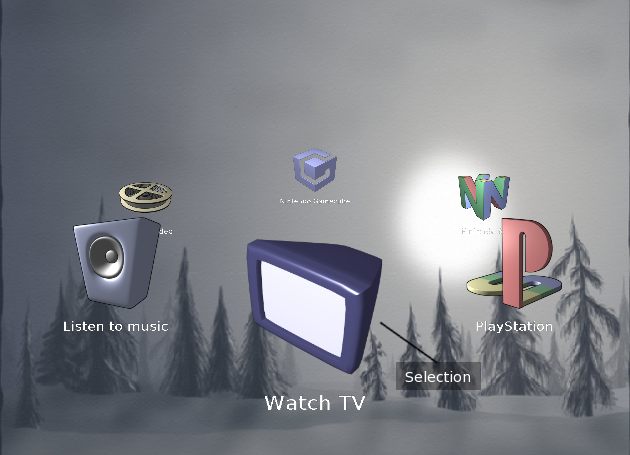
\includegraphics[width=4in]{figures/ring_menu}
\caption{Main ring menu interface\label{figure:RingMenu}}
\end{figure}

The ring menu provides several advantages over a normal list.  It is
immediately obvious to the user which item is selected because of how items
are sized and placed on the screen.  In addition to visual feedback, the ring
menu provides extremely natural interaction; it is very intuitive to navigate
between menu items, even in the absence of a pointing device.  Finally,
because the ring can rotate in either direction, the maximum number of input
``clicks'' is $n \over 2$.  Because every item is visible on the screen at the
same time, the ring layout is suitable only for menus with a small number
of items; tests during prototyping showed that with more than seven or eight
items, the ring layout became too visually cluttered to be useful.

The ring menu responds to several events.  These events correspond to button
presses on a remote control or key presses on the keyboard.  When the ring
menu receives an event corresponding to the ``enter'' button, it activates the
current item. When it receives an ``escape'' event, it deactivates the menu.
These two buttons are used the same in all of the following menus as well in
order to provide a consistent interface for the user to navigate through menus.

Ring-menu specific interaction is handled through the ``right'' and ``left''
buttons.  When the user presses one of these, the ring spins clockwise or
counter-clockwise, respectively.  Each button press moves one item in that
direction.

\subsection{Arc Menu}
The arc menu, shown in Figure \ref{figure:ArcMenu}, is one of the two menu
interfaces designed for larger capacity.  It is similar to the ring menu in
that the selected item is shown centered and with the largest size while other
items are sized with regards to the ``distance'' away from the selection.
This exponential sizing and positioning keeps a common paradigm with the ring
menu.

\begin{figure}[htb]
\centering
\includegraphics[width=4in]{figures/arc_menu}
\caption{Arc menu, as designed in the prototype\label{figure:ArcMenu}}
\end{figure}

Unlike the ring menu, the arc menu does not display every single item on the
screen at once.  Instead, it shows only 5 or 7 items, with the others hidden
off-screen.  As the user navigates through the menu, hidden items become
visible at the top or bottom of the screen as others are pushed off.  In this
way, navigating through the menu is intuitively similar to traditional
scrolling.

The arc menu can theoretically contain any number of items, but as the list
gets longer, the time required for the user to find a particular item
increases.  The significant interaction requirements of this are partially
alleviated by the ability to ``page'' through the menu.

As in the ring menu, ``enter'' is used to activate the currently selected item
and ``escape'' is used to deactivate the menu.  Because the menu is oriented
vertically rather than horizontally, ``up'' and ``down'' are used for
single-item navigation.  Because the arc menu may have a large number of items,
two paging buttons are also available: ``right'' behaves like a page-down key
and ``left'' like a page-up.  This provides an easily discoverable method of
navigating quickly through many options.

The arc menu provides a large area to the left of the items for a preview.
This space can be used at the discretion of the particular menu, and this
will be discussed further in section \ref{DefaultUI}.

\subsection{Cityscape Menu}
The cityscape menu, pictured in Figure \ref{figure:CityscapeMenu}, is
specifically designed for situations where a large number of items are
required.  Inspired by the 3D file manager seen in the movie
\textit{Jurassic Park}, the cityscape menu represents items as if they were
buildings in a city.  While the metaphor is relatively superficial, it
is useful for discussion; the user is never told to think of this menu like
a city.

Each building in the cityscape menu represents either an item or group of
items.  These two types are differentiated primarily by color.  In addition,
group items will show their immediate children as smaller buildings on top.
This is visible in the prototyped cityscape, though certainly not perfected.
Only a single-level of children is shown; it communicates to the user that
there is another level of detail there, but showing the entire ``tree'' of
items would just produce useless visual clutter.

\begin{figure}[htb]
\centering
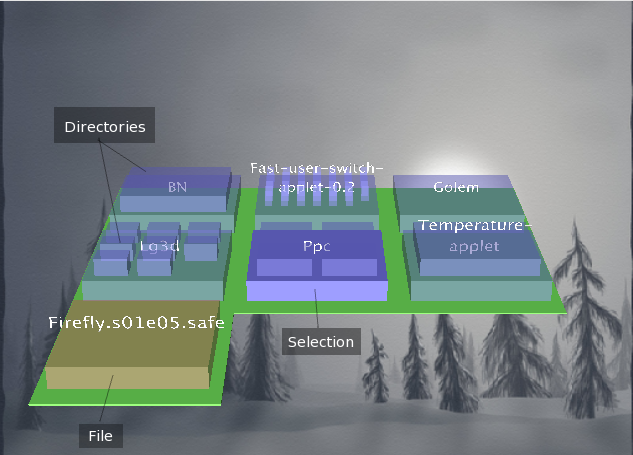
\includegraphics[width=4in]{figures/city_menu}
\caption{Cityscape menu showing the local filesystem\label{figure:CityscapeMenu}}
\end{figure}

The cityscape responds to ``enter'' and ``escape'' somewhat differently from
the ring and arc menus.  When a non-group item is selected, ``enter'' activates
the item as expected.  However, if a group item is selected, ``enter'' zooms
the view into that group so that the items within it can be selected.  When
the view is zoomed into a group, ``escape'' will zoom out a level.  If the
current view is at the highest level, ``escape'' deactivates the menu.

To navigate the cityscape, the user can use all four of the directional buttons.
The cityscape menu is laid out as a two-dimensional array of buildings.
The arrow keys move the selection one item in the particular direction.

The cityscape menu has a particular strength for representing huge numbers of
items.  Because items are effectively laid out in three dimensions (depth
of the zoom plus the two-dimensional building layout), the number of input
clicks to navigate to a particular item is dramatically reduced.  The drawback
to this approach is that an individual item cannot display very much
information about itself.

\section{Default User Interface}
\label{DefaultUI}
These three menu types are used to assemble \textit{smrt}'s user interface.
While the particular use of these menus is left up to the user (see
section \ref{MenuConfig}), they were designed with particular use cases in
mind.  The following sections discuss these uses an explain how a typical
\textit{smrt} session might look.

\subsection{Menu Stack}
At the core of \textit{smrt}'s user interface is the idea of a menu stack.
Because \textit{smrt} covers many different functions -- it can play music,
watch movies, record television, etc. -- there is no ``default state.''  Other
similar systems such as cable boxes default to displaying live TV, but doing
this in \textit{smrt} makes an assumption about the usage preferences of the
user, which is something that the architecture tries to avoid.

Instead, \textit{smrt} begins with a \textit{main menu} from which the user
can select functionality.  This menu cannot be deactivated.  When an item
is selected, it is effectively pushed onto the stack.  If the item is a menu,
it will be displayed until it is either deactivated or something else is
pushed on top of it.  If the item results in an application being launched,
that application will occupy the top of the stack until it quits.  When menus
are deactivated, they are popped off the stack.

By organizing menus in this way, \textit{smrt} provides a flexible yet
consistent way for users to assemble and navigate their media center.  Because
navigation within the stack is constrained, there is no way for a user to
get the system into a state from which they cannot escape; it is always
possible to navigate back to the main menu and start over.

\subsection{Default Menu Configuration}
If the user chooses not to modify \textit{smrt}'s user interface, they will be
presented with the following menu hierarchy. This default configuration is
intended to provide all the functionality a user might want from the software in
a sane fashion.

When \textit{smrt} first starts up, the user is presented with a main menu.
The main menu is a ring menu that presents the user with a few simple actions:
Listen to Music, Watch a Video, Watch TV. Additionally, if there is a DVD in the
DVD drive there will be a ``Watch a DVD'' option. Similarly, if there is an
audio CD in the drive there will be a ``Listen to a CD'' option in the main
menu.

When the user selects the ``Listen to Music'' option they are taken to a
cityscape menu. This menu display the contents of a directory containing music
files (mp3's, ogg's, \textit{etc}.). The user can then browse their music
collection using the remote or keyboard and select music for playback.
Similarly, when the user selects ``Watch a Video'' they are taken to a cityscape
menu displaying the contents of a directory containing video files (avi's,
mpg's, \textit{etc}.). Selecting a video here causes it to start playing.
Quitting either the audio or video playback takes the user back to the directory
where they selected the file. From their they can navigate to other files for
playback, or they can navigate back to the main menu by pressing escape.

Selecting ``Watch TV'' takes the user to an arc menu displaying a list of TV
channels. To the left of the menu is a ``preview'' area that displays the
selected TV channel.  Below the preview area is some program information telling
the user what is currently on, some programs that will run in the near future,
and the times and durations of these programs. This menu allows the user to
simultaneously surf the available channels and get program information about the
available channels. Activating a channel from the arc menu causes that channel to
be displayed full-screen. After activating a channel the user can press escape to
return to the arc menu. The channel they had just been watching will be
selected in the arc menu, its contents displayed in the preview area.

Finally, selecting either ``Watch a DVD'' or ``Listen to a CD'' when there is a
disc in the drive will cause the disc to begin playing. Exiting the playback
with the escape button brings the user back to the main menu. Ejecting the disc
from the drive causes these menu items to be removed from the main menu.

% NOTE: "menu" and "application" are capitalized correctly here because they
%       refer to the packages, not the classes.
\section{Design Overview}
\label{DesignOverview}
\textit{smrt}'s code can be divided coarsely into four modules (Figure
\ref{fig:modules}): the state controller, the application manager, menus, and
applications. The state controller tracks internal state changes. The
application manager handles interaction with external applications such as media
players. The state controller and the application manager are created by the
\texttt{MediaCenter} class when \textit{smrt} is started. The \texttt{menu}
package implements \textit{smrt}'s three basic menu types: ring, arc, and
cityscape. In addition, it contains some specialized subclasses of these menu
types for implementing specific behavior, such as a cityscape which browses the
filesystem.  The \texttt{application} package represents external applications
internally for the state controller.

\begin{figure}[htb]
\centering
\includegraphics[height=.9\linewidth,angle=-90]{figures/modules}
\caption{A high-level conception of \textit{smrt}'s four primary
modules.\label{fig:modules}}
\end{figure}

\subsection{The State Controller}
The state controller, shown in Figure \ref{fig:MediaCenter}, is a singleton
created when \textit{smrt} is started by the \texttt{MediaCenter} class.  The
\texttt{StateController} class has two functions. First, it tracks state changes
so that the user can always return to the previous state. Second, it receives
events from Looking Glass which it passes to the current state, either a menu or
application, to be processed.  To accomplish both of these tasks the
\texttt{StateController} class makes use of the \texttt{Context} interface.

\begin{figure}[htb]
\centering
\includegraphics[height=.9\linewidth,angle=-90]{figures/MediaCenter-uml}
\caption{The \texttt{MediaCenter} class creates the \texttt{StateController}
and \texttt{ApplicationManager}.\label{fig:MediaCenter}}
\end{figure}

The state controller maintains a stack of \texttt{Context} objects for the
purpose of tracking current and previous states. All menu and application
classes implement the \texttt{Context} interface (Figure \ref{fig:Context}).
This allows menus and applications to occupy the screen and receive events.
Every time a new menu or application is displayed, it is pushed onto the top
of the stack.  The previous menu is restored by simply popping off the top
of the stack.

For example, when the user selects a video file from a menu, the video is
launched in a media player.  This media player becomes the current context and
is pushed onto the stack in the \texttt{StateController}.  When the video ends
or the user stops the media player, the \texttt{Context} that represented the
media player is removed from the stack and the menu below -- the one from which
the user selected the file -- is restored as the current context.

When \texttt{MediaCenter} creates the \texttt{StateController}, it tells the
state controller to push the main menu onto its stack, making the main menu the
current context. The state controller will not allow this context to be popped
off of the stack. This ensures that the user cannot put \textit{smrt} into a
state where it has no context.

\begin{figure}[htb]
\centering
\includegraphics[height=.9\linewidth,angle=-90]{figures/Context-uml}
\caption{The \texttt{Context} interface.\label{fig:Context}}
\end{figure}

In addition to helping the state controller track state changes, the
\texttt{Context} interface provides a mechanism for the
\texttt{StateController} class to communicate events to menus and applications.
Whenever the \texttt{StateController} receives an event from Looking Glass, it
passes that event to the current context using the \textbf{processEvent}()
method. The current state, the \texttt{Context} that has control at that
moment, can then handle the event or ignore it. Hitting ``q'' while a video is
playing, for instance, might cause the player to quit. However, hitting ``q''
in a menu will have no effect. All event handling is implemented by the object
that represents \textit{smrt}'s current state, but these \texttt{Context}s are
not directly connected to Looking Glass to receive the events. This way there
is no need to complicate the implementation of a particular \texttt{Context}
to handle connecting and disconnecting event listeners whenever the context
changes.  In fact, a \texttt{Context} has no knowledge of whether or not it is
displayed to the user.

\subsection{The Application Manager}
The application manager keeps track of all the external applications that
\textit{smrt} uses. It associates applications with file types so that when a
user selects a file, \textit{smrt} can launch the appropriate application. The
\texttt{ApplicationManager} class uses a hash map to map regular expressions to
application factories. Application factories, shown in Figure
\ref{fig:ApplicationFactory}, are used to create instances of the
\texttt{Application} class -- or rather, instances of a subclass of
\texttt{Application}. \texttt{ApplicationFactory}s are added to the hash map
with the \textbf{registerApplication}() function. The process of mapping file
extensions to applications is explained further in section \ref{AppConfig}.

\begin{figure}[htb]
\centering
\includegraphics[height=.9\linewidth,angle=-90]{figures/ApplicationFactory-uml}
\caption{The \texttt{ApplicationFactory} launches external applications for
\textit{smrt}.\label{fig:ApplicationFactory}}
\end{figure}

\subsection{Menus}
Menus are the heart of \textit{smrt}'s user interface. Figure \ref{fig:Menu}
shows the class hierarchy for menus. All menus inherit from an abstract base
class, \texttt{Menu}, that implements the \texttt{Context} interface.  Each
\texttt{Menu} subclass is responsible for tracking the items in the menu,
handling event processing, and displaying the menu items on screen. Menu
classes use a layout class to position their items on screen. The layout
classes position menu items on screen according to the menu type; so for each
menu type -- ring, arc, and cityscape -- there is a corresponding layout class
that displays the menu's items on the screen. The \texttt{RingLayout} class,
for example, places the items in a \texttt{RingMenu} on screen in a circle, as
shown in Figure \ref{figure:RingMenu}. When a menu receives an event that
should change which menu item is currently selected, the menu instructs its
layout class to move its menu items to reflect this change.  This is
effectively a Looking Glass implementation detail, but it makes it possible
to create specialized subclasses of a menu type without worrying about
reimplementing the layout mechanisms.

\begin{figure}[htb]
\centering
\includegraphics[height=.9\linewidth,angle=-90]{figures/Menu-uml}
\caption{\textit{smrt}'s menu class hierarchy.\label{fig:Menu}}
\end{figure}

Special purpose menus (the \texttt{TvArcMenu} and \texttt{FilesystemCity} in
Figure \ref{fig:Menu}) subclass one of the concrete menu classes to implement
their own functionality using one of the three menu layouts. These menus differ
from their parents by how they populate themselves with menu items. Most
\texttt{Menu} subclasses are populated with items specified by an XML file (see
Section \ref{MenuConfig}). These special purpose menus do not however.  Rather,
they override their parent's \textbf{realize}() method to populate themselves
when they are displayed. For example the cityscape menu, used for browsing the
file system, must create menu items from files and directories in a given root
directory.  It would be unreasonable to expect the user to produce an XML file
specifying their entire file system.

\subsection{Applications}
\textit{smrt} keeps track of applications it starts using the
\texttt{Application} class. For each external application that \textit{smrt}
uses, there is a subclass of this abstract application class (Figure
\ref{fig:Application}). An instance of one of \texttt{Application}'s subclasses
represents an application running in a separate thread. These objects allow
\textit{smrt} to pass commands to the application.

\begin{figure}[htb]
\centering
\includegraphics[height=.9\linewidth,angle=-90]{figures/Application-uml}
\caption{\textit{smrt}'s internal representation of applications.\label{fig:Application}}
\end{figure}

\section{Classes}
\label{Classes}
This section provides a detailed description of the classes which implement the
core functionality of \textit{smrt}.  Each class description begins with a
brief discussion of the purpose of the class, along with an explanation of its
interactions.  Following this is a precise definition of each of the methods
important to these interactions.

\subsection{StateController}
The \texttt{StateController} is responsible for maintaining the \texttt{Context}
stack and routing events.  It also implements the singleton design pattern, in
order to make it extremely easy to manipulate the state of \textit{smrt} from
anywhere in the application without passing around a handle to the
\texttt{StateController}.  In addition, it also responds to \textit{actions},
which tell the \texttt{StateController} how to modify the current state.

\begin{itemize}
\item[] static \textbf{StateController getInstance} ()
\begin{quotation}
Return the \texttt{StateController} instance.  Implementation of this method
fulfills the singleton pattern.
\end{quotation}

\item[] \textbf{void action} (\textbf{String} \textit{action}, \textbf{String} \textit{arg})
\begin{quotation}
Interpret a text-encoded action.  These actions are the primary way that menus
define the behavior of their items.  There are currently two actions defined:
``push'' and ``launch.''  When the \texttt{StateController} receives a ``push''
action, it loads the menu defined in the file given as \textit{arg} using the
\texttt{MenuLoader} and pushes it on the stack.  When it receives a ``launch''
action, it asks the \texttt{ApplicationManager} to launch the
\texttt{Application} which handles the string given in \textit{arg}.
\end{quotation}

\item[] \textbf{void push} (\textbf{Context} \textit{context})
\begin{quotation}
Push \textit{context} onto the top of the stack.  This causes the current
\textbf{Context} to be hidden, and \textit{context} to be shown.
% When this occurs, the
% \texttt{StateController} also needs to change the visibility of whichever
% item occupies the top of the stack in order to hide it before
% \textit{context} is shown to the user.
\end{quotation}

\item[] \textbf{void pop} ()
\begin{quotation}
Pop the top of the \texttt{Context} stack off, restoring item visibility as
necessary.  If this operation would result in a pop of the lowest-level of the
stack, then this method does nothing.
\end{quotation}

\item[] \textbf{void pop} (\textbf{Context} \textit{test})
\begin{quotation}
Pop the top of the \texttt{Context} stack only if the top is \textit{test}.
This is necessary because all \texttt{Application} instances will call
\textbf{pop}() when the process quits, regardless of whether or not the
Application occupies a spot on the stack.
\end{quotation}
\end{itemize}

\subsection{Context}
\texttt{Context} is the basic interface implemented by the \texttt{Menu} and
\texttt{Application} classes.  By implementing this interface, a class is
allowed to occupy a place on the main interface stack in the
\texttt{StateController}.  If a \texttt{Context} occupies the top of the stack,
that \texttt{Context} will receive events.

\begin{itemize}
\item[] \textbf{void processEvent} (\textbf{LgEvent} \textit{event})
\begin{quotation}
Handle the \textit{event} based on the particular behavior of a given
\texttt{Context}. For instance, a menu may react to particular arrow keys or
enter events through this mechanism.
\end{quotation}
\end{itemize}

\subsection{application.Application}
\textit{smrt} requires an internal representation of all the applications it
uses in order to control them. The \texttt{Application} class is an abstract
base class for all such representations. For every application used by
\textit{smrt} there is a subclass of \texttt{Application} to represent it.  This
class provides functions for starting instances of an application.  Because of
the way that Java's \texttt{Process} class works, \texttt{Application} extends
Java's \texttt{Thread} class so that there can be reliable notification when
the process quits.  An instance of an \texttt{Application} subclass directly
represents a running or completed process.

When the process completes, an \texttt{Application} should notify the
\texttt{StateController} by calling \textbf{pop} (\textit{this}).

\begin{itemize}
\item[] \textbf{void run} ()
\begin{quotation}
Executes the application represented by this object, in a separate thread.
\end{quotation}
\end{itemize}

\subsection{application.ApplicationFactory}
The \texttt{ApplicationFactory} is used to create \texttt{Application} objects
and launch the applications in a different thread. In addition to subclassing
\texttt{Application}, each application used by \textit{smrt} has a subclass of
\texttt{ApplicationFactory}.  This is done because some applications may
require additional environment or command-line arguments beyond a filename.

\pagebreak %hack to get page-break right

\begin{itemize}
\item[] \textbf{public String[]} \textit{regexs}
\begin{quotation}
This is an array of regular expressions which this ApplicationFactory will
be responsible for.  If the \texttt{StateController} receives a ``launch''
command and the argument to that command matches one of the expressions in
\textit{regexs}, this factory's \textbf{launch} method will be called.
\end{quotation}
\item[] \textbf{Application launch} (\textbf{String} \textit{arg})
\begin{quotation}
Returns an \texttt{Application} object corresponding to a running process. The
application is launched with \textit{arg} as its arguments.
\end{quotation}
\end{itemize}

\subsection{application.ApplicationManager}
\textit{smrt}'s use of external applications is overseen by the
\texttt{ApplicationManager}. Like the \texttt{StateController} class, this class
is a singleton. It maps regular expressions to instances of
\texttt{ApplicationFactory}. When a file matches a pattern, the
\texttt{ApplicationManager} uses the corresponding factory to launch the
application assigned to that file type.

\begin{itemize}
\item[] \textbf{void registerApplication} (\textbf{ApplicationFactory} \textit{factory})
\begin{quotation}
Adds a new \texttt{ApplicationFactory} to the known factories so that
applications of this type may be launched.
% Stores
% \textit{factory} in a \texttt{HashMap} with the compiled regular expressions
% from \textit{factory} as the keys.
\end{quotation}

\item[] \textbf{Application launch} (\textbf{String} \textit{arg})
\begin{quotation}
Launch an application configured for use with the file type of the file
specified by \textit{arg}. If there is no \texttt{ApplicationFactory} registered
with the \texttt{ApplicationManager} for this file type, an exception is thrown.
% If \textit{arg} matches one of the keys in the \texttt{HashMap} of factories,
% \textbf{launch} uses that factory to start the application.
\end{quotation}
\end{itemize}

\subsection{menu.Menu}
\texttt{Menu} is the abstract class of which all other \texttt{Menu}s are
children.  It maintains an ordered collection of items and provides the
functionality to add, get a copy and remove these items.  It implements
\texttt{java.io.Serializable} to allow the use of XML files to populate the
menus, discussed bellow.  It also implements \texttt{Context}, so that any
subclass of \texttt{Menu} can be stored in the \texttt{StateController}s main
stack.

\begin{itemize}
\item[] \textbf{void addItem} (\textbf{Item} \textit{item})
\begin{quotation}
Add \textit{item} to the end of this \texttt{Menu}'s collection of
\textbf{Items}.
\end{quotation}

\item[] \textbf{void removeItem} (\textbf{Item} \textit{item})
\begin{quotation}
Remove \textit{item} from this \texttt{Menu}'s collection of \textbf{Item}s.
\end{quotation}

\item[] \textbf{Item getItem} (\textbf{int} \textit{index})
\begin{quotation}
Returns the \textbf{Item}, located at position \textit{index} in this
\texttt{Menu}'s collection of \textbf{Item}s.
\end{quotation}
\end{itemize}

\subsection{menu.Item}
\texttt{Item} is the abstract class from which all menu items, that is all
objects that can be manipulated by the \texttt{Menu} class, inherit.  It has
variables to maintain its name, its associated action, and that action's
associated arguments. In general, these are expected to be set from an XML file
and therefore \texttt{Item} contains several methods used exclusively for
XML decoding.  \texttt{Item} and its children are the only type of objects
that a \texttt{Menu} class can maintain.

\begin{itemize}
\item[] \textbf{void activate} ()
\begin{quotation}
Performs \texttt{Item}'s \textit{action}.
% It first gets a reference
% o the \texttt{StateController}, of which there is only one. It then calls
% texttt{StateController}'s \textbf{action} method with \texttt{Item}s
% textit{action} and \textit{actionArgument} as parameters.
\end{quotation}
\end{itemize}

\subsection{menu.CityLayout}
\texttt{CityLayout} is a generic layout class that is in charge of arranging and
displaying the items in the menu.  It implements \texttt{LayoutManager3D} and
works similar to the other menu layout classes, with additional support for
semaphores (to support asynchronous changes to the layout).

\begin{itemize}
\item[] \textbf{void takeSemaphore} ()
\begin{quotation}
Increase the class's semaphore usage count, preventing updates to the layout
to all other classes besides the requester.  If a class has the layout locked
with an existing semaphore, it delays in a ready-wait loop until the semaphore
is returned.
\end{quotation}

\item[] \textbf{void giveSemaphore} ()
\begin{quotation}
Return a semaphore taken by a class.  This allows other classes to lock the
layout for their own use, or otherwise unlocks the layout.
\end{quotation}
\end{itemize}

\subsection{menu.FilesystemCity}
\texttt{FilesystemCity} is a special-case subclass of the \texttt{CityScape} that
populates itself from the user's local filesystem.  It inherits from the
\texttt{CityScape} class to provide the core functionality of drawing and
navigation, but in addition implements some extra functionality.  This functionality
includes support for asynchronously loading files and directories and displaying
them in the menu as the items are retrieved.  Additionally, filenames are filtered
to show only the type of files needed for the particular menu (such as movies or
music files) as well as print the names of the files in a more human-readable form.

\begin{itemize}
\item[] \textbf{void setFilters} (\textbf{String}[] \textit{filters})
\begin{quotation}
Sets the filters for the \texttt{FilesystemCity}. \textit{filters} is a list of
the patterns used to filter strings. Any filename matching one of the filters in
\textit{filters} will be displayed.
% Given a list of class names, this function sets up filters that are used to format
% and determine which file types get displayed in the menu.  For each class name
% specified, it creates a new instance and adds it to the \texttt{FilesystemCity}'s
% filters list.  During menu population, this list of filters is used
% to determine which files to display.  If any filter determines that the file should
% not be displayed, then the menu will not display it as an option.
\end{quotation}

\item[] \textbf{void setRoot} (\textbf{String} \textit{root})
\begin{quotation}
Sets the \textit{FilesystemCity}'s root directory.  The menu starts from this directory,
listing its files and directories in the menu.  From there, the user can navigate into
lower-level directories.
\end{quotation}
\end{itemize}

\subsubsection{menu.FilesystemCity.DirectoryCrawler}
The \texttt{DirectoryCrawler} is a class implemented within the \texttt{FilesystemCity}
class that takes the responsibility of crawling a user's filesystem for entries.  It
inherits from the \texttt{Thread} class, allowing it to search and populate while the menu is
displayed.

\begin{itemize}
\item[] \textbf{void run} ()
\begin{quotation}
The \texttt{Thread} class implementation of the \textbf{run} () function.  This function
is responsible for crawling the filesystem and adding any file or directory buildings
to the menu as necessary.  It uses the \texttt{FilesystemCity} parent class's
\textbf{filters} list to generate the list of appropriate files and directories to display.
Then, it creates new buildings for them, adds them to the layout, and renders them.
\end{quotation}
\end{itemize}

\subsection{menu.filter.FilenameFilter}
\texttt{FilenameFilter} is an abstract base class for implementing classes that
modify the names of files before they are displayed on the screen.  Currently
the only implementation of this class is \texttt{PrettyPrint}, which removes
file extensions, converts underscores to spaces, and capitalizes individual
words -- for example, changing ``101\_the\_cage.avi'' to ``101 The Cage''.
These filters are attached to a \texttt{FilesystemCity} inside the XML
configuration.

\begin{itemize}
\item[] \textbf{String filter} (\textbf{String} \textit{path}, \textbf{String} \textit{name})
\begin{quotation}
Rewrite the filename given in \textit{name} according to the particular filter.
The full path of the file is given as well, in case the filter wishes to take
that into account.
\end{quotation}
\end{itemize}

\subsection{menu.Directory}
The \texttt{Directory} class extends the \texttt{Building} class for the cityscape
menu.  For the most part, it is exactly the same as \texttt{Building}, but
it implements a feature for displaying sublevels of items on top of its own
item.  This allows users to get a feel for how many objects are contained
within the directory represented by this class.

\begin{itemize}
\item[] \textbf{void setPath} (\textbf{String} \textit{path})
\begin{quotation}
Set the filesystem path that this directory represents.
\end{quotation}

\item[] \textbf{String getPath} ()
\begin{quotation}
Retrieve the path that this directory represents.
\end{quotation}

\pagebreak % another page-break hack

\item[] \textbf{void createSubItems} (\textbf{int} \textit{items})
\begin{quotation}
Called by the function populating the menu.  This tells the directory how many
objects it should show in its sublevel, and performs the required drawing
operations.
\end{quotation}

\item[] \textbf{void realizeSublevel} ()
\begin{quotation}
Perform the necessary calculations and object creation to display sublevel items
on top of the directory object.  The items are arranged similarly to how the
cityscape menu itself is arranged.  This allows the sublevel to graphically
change into the main level when selected, as the cityscape will zoom in on
the sublevel.
\end{quotation}
\end{itemize}

\section{File Formats}
\label{FileFormats}
\textit{smrt} makes very few assumptions about the configuration and layout of
the user's environment.  Instead, it allows the user to customize
\textit{smrt}'s behavior to match their environment through a few simple XML
files.  The basic format of these files is JavaBeans XML
\footnote{\url{http://java.sun.com/products/jfc/tsc/articles/persistence3/}},
and so only the contents of the files are described here rather than the format.

%Maybe I don't know exactly how this works
\subsection{Menu Configuration}
\label{MenuConfig}
Menus in \textit{smrt} are usually created entirely using XML.  This allows a
user to customize the \textit{smrt} installation to match their existing
hardware, media collection and personal preferences remarkably easily.  At
system start-up, \textit{smrt} pushes the menu described in
\textit{main-menu.menu} onto the stack.  Beyond this point, all menu
functionality is determined by the menu configuration.
%What exactly is the "menu configuration" Are menus ALWAYS created entirely
%using XML or mostly

The basic format of a .menu file is JavaBeans XML, with a single object of any
\texttt{Menu} subclass and zero or more \texttt{Item} objects.  For entirely
user-defined menus, each of the items will be listed in this file.  However,
there are situations in which it is impractical for every item to be created by
hand (a file-system CityScape for example).  For this reason, some \texttt{Menu}
subclasses populate themselves based on data configured in this .menu file.
%In what file? .menu?

For a basic menu, the .menu file specifies which items to populate the menu with
and what action to associate with each \texttt{Item}.  The basic
\texttt{IconItem} object has several properties, including a label, an image
file and an \textit{action}. The action tells \textit{smrt} how to behave when
the a given \texttt{Item} is selected.

In the following example, the user wishes to display two items in the ring
menu; a TV item that loads the menu defined in ``tv.menu'' and a DVD item which
tells \textit{smrt} to launch whichever application is set to handle the string
``dvd://''.  This application configuration is described in the next section.

\begin{verbatim}
<java version="1.5.0" class="java.beans.XMLDecoder">
    <object class="org.jdesktop.lg3d.apps.smrt.menu.RingMenu"/>
    <object class="org.jdesktop.lg3d.apps.smrt.men.IconItem">
        <void property="iconFilename">
            <string>home/filePath/tvImage.png</string>
        </void>
        <void property="iconAspect">
            <float>1.0</float>
        </void>
        <void property="label">
            <string>Watch TV</string>
        </void>
        <void property="action">
            <string>push</string>
        </void>
        <void property="actionArgument">
            <string>tv</string>
        </void>
    </object>
    <object class="org.jdesktop.lg3d.apps.smrt.men.IconItem">
        <void property="iconFilename">
            <string>home/filePath/dvdImage.png</string>
        </void>
        <void property="iconAspect">
            <float>1.0</float>
        </void>
        <void property="label">
            <string>Watch DVD</string>
        </void>
        <void property="action">
            <string>launch</string>
        </void>
        <void property="actionArgument">
            <string>dvd://</string>
        </void>
    </object>
</java>
\end{verbatim}

\subsection{Application Configuration}
\label{AppConfig}
The \textit{applications.conf} file specifies the different applications the
user wants to take advantage of; \textit{smrt} does not implement any playback
functionality itself, choosing alternatively to leverage external existing
applications.  This config file lists \texttt{ApplicationFactory} objects and
configures each with a list of regular expressions which will be used to match
an application to a launch string.

In this example, the user has configured their system to use two different
applications: \textit{Xine} and \textit{MPlayer}.  Each of these applications
has an \texttt{Application} subclass inside the \textit{smrt} implementation, so
those object paths reference \textit{smrt} code.  The user has chosen to use
Xine to play avi and mpeg files, as well as DVDs.  MPlayer is configured to be
used only for live TV playback.

\begin{verbatim}
<java version="1.5.0" class="java.beans.XMLDecoder">
    <object class="org.jdesktop.lg3d.apps.smrt.application.XineFactory">
        <void property="regexs">
            <array class="java.lang.String">
                <string>.*\.avi</string>
                <string>.*\.mpeg</string>
                <string>dvd\://.*</string>
            </array>
        </void>
    </object>
    <object class="org.jdesktop.lg3d.apps.smrt.applciation.MPlayerFactory">
        <void property="regexs">
            <array class="java.lang.String">
                <string>tv\://p{Digit}*</string>
            </array>
        </void>
    </object>
</java>
\end{verbatim}

\section{Summary}
This document broke down and explained \textit{smrt}'s design. From the user
interface to the class implementations and file formats, this document provided
a comprehensive basis and explanation of \textit{smrt}'s implementation.
Sections \ref{UIElements} and \ref{DefaultUI} described the user interface.
First, Section \ref{UIElements} explained the rationale behind each component of
the user interface, and how each component operates. Section \ref{DefaultUI}
showed how the components described in Section \ref{UIElements} combine to
create \textit{smrt}'s user interface.  In Section \ref{DesignOverview}, a
high-level overview of \textit{smrt}'s internal design was provided. It
explained the interaction between the modules that provide for \textit{smrt}'s
functionality. Following this, in Section \ref{Classes}, was a more technical
look at the most significant classes that comprise the modules described in
Section \ref{DesignOverview}.  Finally, Section \ref{FileFormats} explained how
\textit{smrt} uses XML files to configure the behavior of its classes.

\pagebreak
\appendix

\section{Glossary}
A list of terms and acronyms used in this document, along with their
definitions, is provided below.

\begin{tabular}{p{.3\linewidth}p{.6\linewidth}}
	\textbf{avi}			& A video file format			\\
	\textbf{DVD}			& Three letters referring to a type of
					  optical disc storage. (In 1999 the DVD
					  Forum decreed that DVD is not an
					  acronym for anything.)		\\
	\textbf{Java}			& The Java programming language		\\
	\textbf{mpeg}			& A video file format			\\
	\textbf{MPlayer}		& An open source media player		\\
	\textbf{Project Looking Glass}	& Sun Microsystems' experimental 3D
					  desktop environment framework		\\
	\textbf{smrt}			& The Czech word for ``death''. Also the
					  name of this project: a rocking 3D
					  home theater interface		\\
	\textbf{TV}			& TeleVision				\\
	\textbf{Xine}			& An open source media player		\\
	\textbf{XML}			& Extensible Markup Language
\end{tabular}

\section{Related Documents}
\begin{list}{}{
\setlength{\parsep}{1ex}
\setlength{\leftmargin}{0.5in}
\setlength{\itemindent}{-0.5in}
}

\item[] \textbf{[Gosling 05]}

	Gosling, James, Bill Joy, Guy Steele, and Gilad Bracha. \textit{The Java
	Language Reference: Third Edition}. Addison-Wesley, Santa Clara, California, 2005.

	The third edition of the Java language specification.

\item[] \textbf{[Bray 04]}

	Bray, Tim, John Cowan, Eve Maler, et al. \textit{Extensible Markup
	Language (XML) 1.1}. W3C, 2004.

	The World Wide Web Consortium's most recent recommendation regarding the
	XML specification.

\item[] \textbf{[Project Looking Glass]}

	http://lg3d-core.dev.java.net/

	The open source web site for Sun's Project Looking Glass.

\item[] \textbf{[Gamma 95]}

	Gamma, Erich, Richard Helm, Ralph Johnson, and John Vlissides.
	\textit{Design Patterns: Elements of Reusable Object-Oriented
	Software}. Addison-Wesley, 1995.

	The definitive work on design patterns.
\end{list}

\end{document}
